\documentclass[1p]{elsarticle_modified}
%\bibliographystyle{elsarticle-num}

%\usepackage[colorlinks]{hyperref}
%\usepackage{abbrmath_seonhwa} %\Abb, \Ascr, \Acal ,\Abf, \Afrak
\usepackage{amsfonts}
\usepackage{amssymb}
\usepackage{amsmath}
\usepackage{amsthm}
\usepackage{scalefnt}
\usepackage{amsbsy}
\usepackage{kotex}
\usepackage{caption}
\usepackage{subfig}
\usepackage{color}
\usepackage{graphicx}
\usepackage{xcolor} %% white, black, red, green, blue, cyan, magenta, yellow
\usepackage{float}
\usepackage{setspace}
\usepackage{hyperref}

\usepackage{tikz}
\usetikzlibrary{arrows}

\usepackage{multirow}
\usepackage{array} % fixed length table
\usepackage{hhline}

%%%%%%%%%%%%%%%%%%%%%
\makeatletter
\renewcommand*\env@matrix[1][\arraystretch]{%
	\edef\arraystretch{#1}%
	\hskip -\arraycolsep
	\let\@ifnextchar\new@ifnextchar
	\array{*\c@MaxMatrixCols c}}
\makeatother %https://tex.stackexchange.com/questions/14071/how-can-i-increase-the-line-spacing-in-a-matrix
%%%%%%%%%%%%%%%

\usepackage[normalem]{ulem}

\newcommand{\msout}[1]{\ifmmode\text{\sout{\ensuremath{#1}}}\else\sout{#1}\fi}
%SOURCE: \msout is \stkout macro in https://tex.stackexchange.com/questions/20609/strikeout-in-math-mode

\newcommand{\cancel}[1]{
	\ifmmode
	{\color{red}\msout{#1}}
	\else
	{\color{red}\sout{#1}}
	\fi
}

\newcommand{\add}[1]{
	{\color{blue}\uwave{#1}}
}

\newcommand{\replace}[2]{
	\ifmmode
	{\color{red}\msout{#1}}{\color{blue}\uwave{#2}}
	\else
	{\color{red}\sout{#1}}{\color{blue}\uwave{#2}}
	\fi
}

\newcommand{\Sol}{\mathcal{S}} %segment
\newcommand{\D}{D} %diagram
\newcommand{\A}{\mathcal{A}} %arc


%%%%%%%%%%%%%%%%%%%%%%%%%%%%%5 test

\def\sl{\operatorname{\textup{SL}}(2,\Cbb)}
\def\psl{\operatorname{\textup{PSL}}(2,\Cbb)}
\def\quan{\mkern 1mu \triangleright \mkern 1mu}

\theoremstyle{definition}
\newtheorem{thm}{Theorem}[section]
\newtheorem{prop}[thm]{Proposition}
\newtheorem{lem}[thm]{Lemma}
\newtheorem{ques}[thm]{Question}
\newtheorem{cor}[thm]{Corollary}
\newtheorem{defn}[thm]{Definition}
\newtheorem{exam}[thm]{Example}
\newtheorem{rmk}[thm]{Remark}
\newtheorem{alg}[thm]{Algorithm}

\newcommand{\I}{\sqrt{-1}}
\begin{document}

%\begin{frontmatter}
%
%\title{Boundary parabolic representations of knots up to 8 crossings}
%
%%% Group authors per affiliation:
%\author{Yunhi Cho} 
%\address{Department of Mathematics, University of Seoul, Seoul, Korea}
%\ead{yhcho@uos.ac.kr}
%
%
%\author{Seonhwa Kim} %\fnref{s_kim}}
%\address{Center for Geometry and Physics, Institute for Basic Science, Pohang, 37673, Korea}
%\ead{ryeona17@ibs.re.kr}
%
%\author{Hyuk Kim}
%\address{Department of Mathematical Sciences, Seoul National University, Seoul 08826, Korea}
%\ead{hyukkim@snu.ac.kr}
%
%\author{Seokbeom Yoon}
%\address{Department of Mathematical Sciences, Seoul National University, Seoul, 08826,  Korea}
%\ead{sbyoon15@snu.ac.kr}
%
%\begin{abstract}
%We find all boundary parabolic representation of knots up to 8 crossings.
%
%\end{abstract}
%\begin{keyword}
%    \MSC[2010] 57M25 
%\end{keyword}
%
%\end{frontmatter}

%\linenumbers
%\tableofcontents
%
\newcommand\colored[1]{\textcolor{white}{\rule[-0.35ex]{0.8em}{1.4ex}}\kern-0.8em\color{red} #1}%
%\newcommand\colored[1]{\textcolor{white}{ #1}\kern-2.17ex	\textcolor{white}{ #1}\kern-1.81ex	\textcolor{white}{ #1}\kern-2.15ex\color{red}#1	}

{\Large $\underline{12n_{0271}~(K12n_{0271})}$}

\setlength{\tabcolsep}{10pt}
\renewcommand{\arraystretch}{1.6}
\vspace{1cm}\begin{tabular}{m{100pt}>{\centering\arraybackslash}m{274pt}}
\multirow{5}{120pt}{
	\centering
	\includegraphics[width=112pt]{../../../GIT/diagram.site/Diagrams/png/2360_12n_0271.png}\\
\ \ \ A knot diagram\footnotemark}&
\allowdisplaybreaks
\textbf{Linearized knot diagam} \\
\cline{2-2}
 &
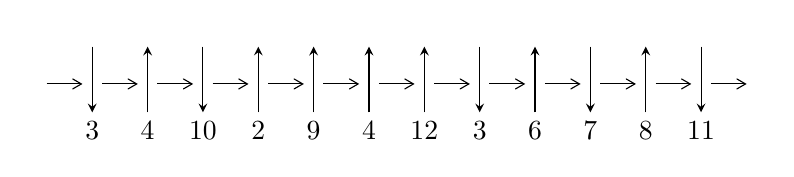
\begin{tikzpicture}[x=20pt, y=17pt]
	% nodes
	\node (C0) at (0, 0) {};
	\node (C1) at (1, 0) {};
	\node (C1U) at (1, +1) {};
	\node (C1D) at (1, -1) {3};

	\node (C2) at (2, 0) {};
	\node (C2U) at (2, +1) {};
	\node (C2D) at (2, -1) {4};

	\node (C3) at (3, 0) {};
	\node (C3U) at (3, +1) {};
	\node (C3D) at (3, -1) {10};

	\node (C4) at (4, 0) {};
	\node (C4U) at (4, +1) {};
	\node (C4D) at (4, -1) {2};

	\node (C5) at (5, 0) {};
	\node (C5U) at (5, +1) {};
	\node (C5D) at (5, -1) {9};

	\node (C6) at (6, 0) {};
	\node (C6U) at (6, +1) {};
	\node (C6D) at (6, -1) {4};

	\node (C7) at (7, 0) {};
	\node (C7U) at (7, +1) {};
	\node (C7D) at (7, -1) {12};

	\node (C8) at (8, 0) {};
	\node (C8U) at (8, +1) {};
	\node (C8D) at (8, -1) {3};

	\node (C9) at (9, 0) {};
	\node (C9U) at (9, +1) {};
	\node (C9D) at (9, -1) {6};

	\node (C10) at (10, 0) {};
	\node (C10U) at (10, +1) {};
	\node (C10D) at (10, -1) {7};

	\node (C11) at (11, 0) {};
	\node (C11U) at (11, +1) {};
	\node (C11D) at (11, -1) {8};

	\node (C12) at (12, 0) {};
	\node (C12U) at (12, +1) {};
	\node (C12D) at (12, -1) {11};
	\node (C13) at (13, 0) {};

	% arrows
	\draw[->,>={angle 60}]
	(C0) edge (C1) (C1) edge (C2) (C2) edge (C3) (C3) edge (C4) (C4) edge (C5) (C5) edge (C6) (C6) edge (C7) (C7) edge (C8) (C8) edge (C9) (C9) edge (C10) (C10) edge (C11) (C11) edge (C12) (C12) edge (C13) ;	\draw[->,>=stealth]
	(C1U) edge (C1D) (C2D) edge (C2U) (C3U) edge (C3D) (C4D) edge (C4U) (C5D) edge (C5U) (C6D) edge (C6U) (C7D) edge (C7U) (C8U) edge (C8D) (C9D) edge (C9U) (C10U) edge (C10D) (C11D) edge (C11U) (C12U) edge (C12D) ;
	\end{tikzpicture} \\
\hhline{~~} \\& 
\textbf{Solving Sequence} \\ \cline{2-2} 
 &
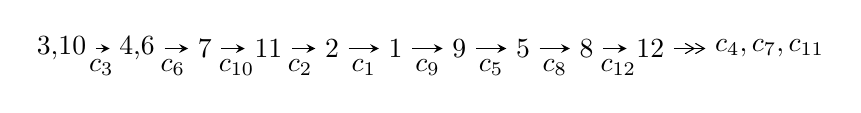
\begin{tikzpicture}[x=23pt, y=7pt]
	% node
	\node (A0) at (-1/8, 0) {3,10};
	\node (A1) at (17/16, 0) {4,6};
	\node (A2) at (17/8, 0) {7};
	\node (A3) at (25/8, 0) {11};
	\node (A4) at (33/8, 0) {2};
	\node (A5) at (41/8, 0) {1};
	\node (A6) at (49/8, 0) {9};
	\node (A7) at (57/8, 0) {5};
	\node (A8) at (65/8, 0) {8};
	\node (A9) at (73/8, 0) {12};
	\node (C1) at (1/2, -1) {$c_{3}$};
	\node (C2) at (13/8, -1) {$c_{6}$};
	\node (C3) at (21/8, -1) {$c_{10}$};
	\node (C4) at (29/8, -1) {$c_{2}$};
	\node (C5) at (37/8, -1) {$c_{1}$};
	\node (C6) at (45/8, -1) {$c_{9}$};
	\node (C7) at (53/8, -1) {$c_{5}$};
	\node (C8) at (61/8, -1) {$c_{8}$};
	\node (C9) at (69/8, -1) {$c_{12}$};
	\node (A10) at (11, 0) {$c_{4},c_{7},c_{11}$};

	% edge
	\draw[->,>=stealth]	
	(A0) edge (A1) (A1) edge (A2) (A2) edge (A3) (A3) edge (A4) (A4) edge (A5) (A5) edge (A6) (A6) edge (A7) (A7) edge (A8) (A8) edge (A9) ;
	\draw[->>,>={angle 60}]	
	(A9) edge (A10);
\end{tikzpicture} \\ 

\end{tabular} \\

\footnotetext{
The image of knot diagram is generated by the software ``\textbf{Draw programme}" developed by Andrew Bartholomew(\url{http://www.layer8.co.uk/maths/draw/index.htm\#Running-draw}), where we modified some parts for our purpose(\url{https://github.com/CATsTAILs/LinksPainter}).
}\phantom \\ \newline 
\centering \textbf{Ideals for irreducible components\footnotemark of $X_{\text{par}}$} 
 
\begin{align*}
I^u_{1}&=\langle 
2.10894\times10^{29} u^{39}+1.76613\times10^{30} u^{38}+\cdots+3.90907\times10^{30} b+1.29800\times10^{31},\\
\phantom{I^u_{1}}&\phantom{= \langle  }-5.78629\times10^{30} u^{39}-1.35625\times10^{31} u^{38}+\cdots+1.95453\times10^{30} a-1.20066\times10^{30},\;u^{40}+2 u^{39}+\cdots-2 u+1\rangle \\
I^u_{2}&=\langle 
b^4-8 b^3 u+4 b^3+2 b^2 u-18 b^2+20 b u-4 b-4 u+7,\;a+u-1,\;u^2- u+1\rangle \\
I^u_{3}&=\langle 
b^3+6 b^2 u+3 b^2-9 b-6 u-3,\;a- u-1,\;u^2+u+1\rangle \\
\\
\end{align*}
\raggedright * 3 irreducible components of $\dim_{\mathbb{C}}=0$, with total 54 representations.\\
\footnotetext{All coefficients of polynomials are rational numbers. But the coefficients are sometimes approximated in decimal forms when there is not enough margin.}
\newpage
\renewcommand{\arraystretch}{1}
\centering \section*{I. $I^u_{1}= \langle 2.11\times10^{29} u^{39}+1.77\times10^{30} u^{38}+\cdots+3.91\times10^{30} b+1.30\times10^{31},\;-5.79\times10^{30} u^{39}-1.36\times10^{31} u^{38}+\cdots+1.95\times10^{30} a-1.20\times10^{30},\;u^{40}+2 u^{39}+\cdots-2 u+1 \rangle$}
\flushleft \textbf{(i) Arc colorings}\\
\begin{tabular}{m{7pt} m{180pt} m{7pt} m{180pt} }
\flushright $a_{3}=$&$\begin{pmatrix}1\\0\end{pmatrix}$ \\
\flushright $a_{10}=$&$\begin{pmatrix}0\\u\end{pmatrix}$ \\
\flushright $a_{4}=$&$\begin{pmatrix}1\\u^2\end{pmatrix}$ \\
\flushright $a_{6}=$&$\begin{pmatrix}2.96044 u^{39}+6.93899 u^{38}+\cdots+26.8232 u+0.614297\\-0.0539500 u^{39}-0.451804 u^{38}+\cdots-0.947110 u-3.32050\end{pmatrix}$ \\
\flushright $a_{7}=$&$\begin{pmatrix}2.92788 u^{39}+6.66255 u^{38}+\cdots+26.8003 u-1.68810\\-0.0424279 u^{39}-0.410687 u^{38}+\cdots-1.33715 u-3.10919\end{pmatrix}$ \\
\flushright $a_{11}=$&$\begin{pmatrix}3.86426 u^{39}+7.66563 u^{38}+\cdots+30.4928 u-10.5738\\0.320422 u^{39}+0.529059 u^{38}+\cdots-0.339238 u-2.95540\end{pmatrix}$ \\
\flushright $a_{2}=$&$\begin{pmatrix}u^2+1\\u^4\end{pmatrix}$ \\
\flushright $a_{1}=$&$\begin{pmatrix}u^4+u^2+1\\u^4\end{pmatrix}$ \\
\flushright $a_{9}=$&$\begin{pmatrix}1.97656 u^{39}+3.87161 u^{38}+\cdots+21.4803 u-4.58523\\0.944726 u^{39}+1.94465 u^{38}+\cdots+5.22209 u-2.88878\end{pmatrix}$ \\
\flushright $a_{5}=$&$\begin{pmatrix}u^4+u^2+1\\u^6+u^2\end{pmatrix}$ \\
\flushright $a_{8}=$&$\begin{pmatrix}2.92129 u^{39}+5.81625 u^{38}+\cdots+26.7024 u-7.47401\\0.944726 u^{39}+1.94465 u^{38}+\cdots+5.22209 u-2.88878\end{pmatrix}$ \\
\flushright $a_{12}=$&$\begin{pmatrix}1.93457 u^{39}+2.86642 u^{38}+\cdots+4.61941 u-15.8609\\-0.942390 u^{39}-2.36759 u^{38}+\cdots-11.6667 u-2.35706\end{pmatrix}$\\&\end{tabular}
\flushleft \textbf{(ii) Obstruction class $= -1$}\\~\\
\flushleft \textbf{(iii) Cusp Shapes $= 3.91026 u^{39}+8.38086 u^{38}+\cdots+29.6027 u+1.57860$}\\~\\
\newpage\renewcommand{\arraystretch}{1}
\flushleft \textbf{(iv) u-Polynomials at the component}\newline \\
\begin{tabular}{m{50pt}|m{274pt}}
Crossings & \hspace{64pt}u-Polynomials at each crossing \\
\hline $$\begin{aligned}c_{1}\end{aligned}$$&$\begin{aligned}
&u^{40}+56 u^{39}+\cdots+84 u+1
\end{aligned}$\\
\hline $$\begin{aligned}c_{2},c_{4}\end{aligned}$$&$\begin{aligned}
&u^{40}-8 u^{39}+\cdots-28 u+1
\end{aligned}$\\
\hline $$\begin{aligned}c_{3}\end{aligned}$$&$\begin{aligned}
&u^{40}+2 u^{39}+\cdots-2 u+1
\end{aligned}$\\
\hline $$\begin{aligned}c_{5},c_{9}\end{aligned}$$&$\begin{aligned}
&u^{40}-3 u^{39}+\cdots+43 u+13
\end{aligned}$\\
\hline $$\begin{aligned}c_{6}\end{aligned}$$&$\begin{aligned}
&u^{40}+4 u^{39}+\cdots+18344 u+4339
\end{aligned}$\\
\hline $$\begin{aligned}c_{7},c_{11}\end{aligned}$$&$\begin{aligned}
&u^{40}- u^{39}+\cdots-12 u+4
\end{aligned}$\\
\hline $$\begin{aligned}c_{8}\end{aligned}$$&$\begin{aligned}
&u^{40}-44 u^{38}+\cdots-2449090 u+232661
\end{aligned}$\\
\hline $$\begin{aligned}c_{10}\end{aligned}$$&$\begin{aligned}
&u^{40}+u^{39}+\cdots-36 u+4
\end{aligned}$\\
\hline $$\begin{aligned}c_{12}\end{aligned}$$&$\begin{aligned}
&u^{40}+25 u^{39}+\cdots+80 u+16
\end{aligned}$\\
\hline
\end{tabular}\\~\\
\newpage\renewcommand{\arraystretch}{1}
\flushleft \textbf{(v) Riley Polynomials at the component}\newline \\
\begin{tabular}{m{50pt}|m{274pt}}
Crossings & \hspace{64pt}Riley Polynomials at each crossing \\
\hline $$\begin{aligned}c_{1}\end{aligned}$$&$\begin{aligned}
&y^{40}-136 y^{39}+\cdots+23220 y+1
\end{aligned}$\\
\hline $$\begin{aligned}c_{2},c_{4}\end{aligned}$$&$\begin{aligned}
&y^{40}+56 y^{39}+\cdots+84 y+1
\end{aligned}$\\
\hline $$\begin{aligned}c_{3}\end{aligned}$$&$\begin{aligned}
&y^{40}+8 y^{39}+\cdots+28 y+1
\end{aligned}$\\
\hline $$\begin{aligned}c_{5},c_{9}\end{aligned}$$&$\begin{aligned}
&y^{40}-5 y^{39}+\cdots+2779 y+169
\end{aligned}$\\
\hline $$\begin{aligned}c_{6}\end{aligned}$$&$\begin{aligned}
&y^{40}+40 y^{39}+\cdots-166465604 y+18826921
\end{aligned}$\\
\hline $$\begin{aligned}c_{7},c_{11}\end{aligned}$$&$\begin{aligned}
&y^{40}+25 y^{39}+\cdots+80 y+16
\end{aligned}$\\
\hline $$\begin{aligned}c_{8}\end{aligned}$$&$\begin{aligned}
&y^{40}-88 y^{39}+\cdots-1066872899128 y+54131140921
\end{aligned}$\\
\hline $$\begin{aligned}c_{10}\end{aligned}$$&$\begin{aligned}
&y^{40}-55 y^{39}+\cdots-112 y+16
\end{aligned}$\\
\hline $$\begin{aligned}c_{12}\end{aligned}$$&$\begin{aligned}
&y^{40}-15 y^{39}+\cdots-2816 y+256
\end{aligned}$\\
\hline
\end{tabular}\\~\\
\newpage\flushleft \textbf{(vi) Complex Volumes and Cusp Shapes}
$$\begin{array}{c|c|c}  
\text{Solutions to }I^u_{1}& \I (\text{vol} + \sqrt{-1}CS) & \text{Cusp shape}\\
 \hline 
\begin{aligned}
u &= -0.764187 + 0.653787 I \\
a &= \phantom{-}0.315530 - 0.761484 I \\
b &= \phantom{-}0.186332 + 0.279615 I\end{aligned}
 & -1.47509 + 2.25056 I & \phantom{-}0.06495 - 2.95440 I \\ \hline\begin{aligned}
u &= -0.764187 - 0.653787 I \\
a &= \phantom{-}0.315530 + 0.761484 I \\
b &= \phantom{-}0.186332 - 0.279615 I\end{aligned}
 & -1.47509 - 2.25056 I & \phantom{-}0.06495 + 2.95440 I \\ \hline\begin{aligned}
u &= -0.213036 + 0.949581 I \\
a &= -0.140457 + 1.057230 I \\
b &= -0.04726 - 2.29506 I\end{aligned}
 & \phantom{-}1.94553 + 4.51368 I & \phantom{-}6.38970 - 7.82355 I \\ \hline\begin{aligned}
u &= -0.213036 - 0.949581 I \\
a &= -0.140457 - 1.057230 I \\
b &= -0.04726 + 2.29506 I\end{aligned}
 & \phantom{-}1.94553 - 4.51368 I & \phantom{-}6.38970 + 7.82355 I \\ \hline\begin{aligned}
u &= \phantom{-}0.955003 + 0.516879 I \\
a &= \phantom{-}0.487517 + 0.951136 I \\
b &= -0.146437 + 0.072845 I\end{aligned}
 & -6.22578 + 0.90518 I & -4.74646 - 0.36762 I \\ \hline\begin{aligned}
u &= \phantom{-}0.955003 - 0.516879 I \\
a &= \phantom{-}0.487517 - 0.951136 I \\
b &= -0.146437 - 0.072845 I\end{aligned}
 & -6.22578 - 0.90518 I & -4.74646 + 0.36762 I \\ \hline\begin{aligned}
u &= -0.444049 + 0.991733 I \\
a &= \phantom{-}0.526547 + 0.513973 I \\
b &= -0.30344 - 1.55709 I\end{aligned}
 & \phantom{-}0.55266 + 1.44737 I & -0.667154 + 0.069332 I \\ \hline\begin{aligned}
u &= -0.444049 - 0.991733 I \\
a &= \phantom{-}0.526547 - 0.513973 I \\
b &= -0.30344 + 1.55709 I\end{aligned}
 & \phantom{-}0.55266 - 1.44737 I & -0.667154 - 0.069332 I \\ \hline\begin{aligned}
u &= \phantom{-}0.670524 + 0.887860 I \\
a &= \phantom{-}0.748302 - 0.870483 I \\
b &= \phantom{-}0.20959 + 1.99021 I\end{aligned}
 & \phantom{-}0.22448 - 2.62080 I & -1.03330 + 3.61519 I \\ \hline\begin{aligned}
u &= \phantom{-}0.670524 - 0.887860 I \\
a &= \phantom{-}0.748302 + 0.870483 I \\
b &= \phantom{-}0.20959 - 1.99021 I\end{aligned}
 & \phantom{-}0.22448 + 2.62080 I & -1.03330 - 3.61519 I\\
 \hline 
 \end{array}$$\newpage$$\begin{array}{c|c|c}  
\text{Solutions to }I^u_{1}& \I (\text{vol} + \sqrt{-1}CS) & \text{Cusp shape}\\
 \hline 
\begin{aligned}
u &= \phantom{-}0.808131 + 0.773706 I \\
a &= \phantom{-}0.177775 + 0.864533 I \\
b &= \phantom{-}0.140485 - 0.763458 I\end{aligned}
 & -3.58036 - 7.21978 I & -1.70984 + 7.47042 I \\ \hline\begin{aligned}
u &= \phantom{-}0.808131 - 0.773706 I \\
a &= \phantom{-}0.177775 - 0.864533 I \\
b &= \phantom{-}0.140485 + 0.763458 I\end{aligned}
 & -3.58036 + 7.21978 I & -1.70984 - 7.47042 I \\ \hline\begin{aligned}
u &= -0.500435 + 1.020290 I \\
a &= -0.288714 + 0.431513 I \\
b &= \phantom{-}0.79094 - 1.35172 I\end{aligned}
 & -0.11396 + 2.62702 I & \phantom{-}1.21166 - 3.80016 I \\ \hline\begin{aligned}
u &= -0.500435 - 1.020290 I \\
a &= -0.288714 - 0.431513 I \\
b &= \phantom{-}0.79094 + 1.35172 I\end{aligned}
 & -0.11396 - 2.62702 I & \phantom{-}1.21166 + 3.80016 I \\ \hline\begin{aligned}
u &= \phantom{-}0.601637 + 0.967840 I \\
a &= -0.452431 - 0.174923 I \\
b &= \phantom{-}0.779446 + 0.975335 I\end{aligned}
 & -2.80937 + 1.79823 I & -2.49074 - 1.24106 I \\ \hline\begin{aligned}
u &= \phantom{-}0.601637 - 0.967840 I \\
a &= -0.452431 + 0.174923 I \\
b &= \phantom{-}0.779446 - 0.975335 I\end{aligned}
 & -2.80937 - 1.79823 I & -2.49074 + 1.24106 I \\ \hline\begin{aligned}
u &= -0.737881 + 0.290228 I \\
a &= \phantom{-}0.95910 + 1.11896 I \\
b &= \phantom{-}0.508089 - 0.650289 I\end{aligned}
 & -1.82966 + 2.58669 I & -3.19003 - 3.49376 I \\ \hline\begin{aligned}
u &= -0.737881 - 0.290228 I \\
a &= \phantom{-}0.95910 - 1.11896 I \\
b &= \phantom{-}0.508089 + 0.650289 I\end{aligned}
 & -1.82966 - 2.58669 I & -3.19003 + 3.49376 I \\ \hline\begin{aligned}
u &= \phantom{-}0.178235 + 0.755403 I \\
a &= -0.004535 - 1.355120 I \\
b &= -0.53972 + 1.87193 I\end{aligned}
 & \phantom{-}2.74915 - 0.87130 I & \phantom{-}9.38374 - 0.76428 I \\ \hline\begin{aligned}
u &= \phantom{-}0.178235 - 0.755403 I \\
a &= -0.004535 + 1.355120 I \\
b &= -0.53972 - 1.87193 I\end{aligned}
 & \phantom{-}2.74915 + 0.87130 I & \phantom{-}9.38374 + 0.76428 I\\
 \hline 
 \end{array}$$\newpage$$\begin{array}{c|c|c}  
\text{Solutions to }I^u_{1}& \I (\text{vol} + \sqrt{-1}CS) & \text{Cusp shape}\\
 \hline 
\begin{aligned}
u &= \phantom{-}0.526875 + 1.146360 I \\
a &= -0.507182 - 0.577873 I \\
b &= \phantom{-}1.35004 + 1.47812 I\end{aligned}
 & -3.91478 - 6.46553 I & -1.90714 + 6.14891 I \\ \hline\begin{aligned}
u &= \phantom{-}0.526875 - 1.146360 I \\
a &= -0.507182 + 0.577873 I \\
b &= \phantom{-}1.35004 - 1.47812 I\end{aligned}
 & -3.91478 + 6.46553 I & -1.90714 - 6.14891 I \\ \hline\begin{aligned}
u &= -0.332002 + 0.640935 I \\
a &= \phantom{-}0.522256 - 0.170528 I \\
b &= \phantom{-}0.045479 - 0.256841 I\end{aligned}
 & -0.02195 + 1.48740 I & \phantom{-}0.17371 - 4.94146 I \\ \hline\begin{aligned}
u &= -0.332002 - 0.640935 I \\
a &= \phantom{-}0.522256 + 0.170528 I \\
b &= \phantom{-}0.045479 + 0.256841 I\end{aligned}
 & -0.02195 - 1.48740 I & \phantom{-}0.17371 + 4.94146 I \\ \hline\begin{aligned}
u &= \phantom{-}1.030620 + 0.897013 I \\
a &= -1.173260 - 0.172864 I \\
b &= \phantom{-}0.179150 - 1.015860 I\end{aligned}
 & -11.47200 + 0.66922 I & \phantom{-0.000000 } 0 \\ \hline\begin{aligned}
u &= \phantom{-}1.030620 - 0.897013 I \\
a &= -1.173260 + 0.172864 I \\
b &= \phantom{-}0.179150 + 1.015860 I\end{aligned}
 & -11.47200 - 0.66922 I & \phantom{-0.000000 } 0 \\ \hline\begin{aligned}
u &= -1.073240 + 0.852439 I \\
a &= -1.229830 + 0.153303 I \\
b &= -0.092752 + 1.188350 I\end{aligned}
 & -15.3931 - 6.0460 I & \phantom{-0.000000 } 0 \\ \hline\begin{aligned}
u &= -1.073240 - 0.852439 I \\
a &= -1.229830 - 0.153303 I \\
b &= -0.092752 - 1.188350 I\end{aligned}
 & -15.3931 + 6.0460 I & \phantom{-0.000000 } 0 \\ \hline\begin{aligned}
u &= \phantom{-}0.926096 + 1.056710 I \\
a &= \phantom{-}0.023831 + 1.156260 I \\
b &= -1.21185 - 2.24051 I\end{aligned}
 & -10.92760 - 7.82692 I & \phantom{-0.000000 } 0 \\ \hline\begin{aligned}
u &= \phantom{-}0.926096 - 1.056710 I \\
a &= \phantom{-}0.023831 - 1.156260 I \\
b &= -1.21185 + 2.24051 I\end{aligned}
 & -10.92760 + 7.82692 I & \phantom{-0.000000 } 0\\
 \hline 
 \end{array}$$\newpage$$\begin{array}{c|c|c}  
\text{Solutions to }I^u_{1}& \I (\text{vol} + \sqrt{-1}CS) & \text{Cusp shape}\\
 \hline 
\begin{aligned}
u &= -1.04261 + 0.96199 I \\
a &= -1.160190 + 0.237458 I \\
b &= \phantom{-}0.515590 + 1.140420 I\end{aligned}
 & -15.7491 + 4.5181 I & \phantom{-0.000000 } 0 \\ \hline\begin{aligned}
u &= -1.04261 - 0.96199 I \\
a &= -1.160190 - 0.237458 I \\
b &= \phantom{-}0.515590 - 1.140420 I\end{aligned}
 & -15.7491 - 4.5181 I & \phantom{-0.000000 } 0 \\ \hline\begin{aligned}
u &= -0.90713 + 1.09807 I \\
a &= -0.010802 - 1.172610 I \\
b &= -1.27643 + 2.56164 I\end{aligned}
 & -14.5518 + 13.2615 I & \phantom{-0.000000 } 0 \\ \hline\begin{aligned}
u &= -0.90713 - 1.09807 I \\
a &= -0.010802 + 1.172610 I \\
b &= -1.27643 - 2.56164 I\end{aligned}
 & -14.5518 - 13.2615 I & \phantom{-0.000000 } 0 \\ \hline\begin{aligned}
u &= -0.98478 + 1.04683 I \\
a &= \phantom{-}0.065240 - 1.184100 I \\
b &= -1.50476 + 1.94665 I\end{aligned}
 & -15.4588 + 2.8896 I & \phantom{-0.000000 } 0 \\ \hline\begin{aligned}
u &= -0.98478 - 1.04683 I \\
a &= \phantom{-}0.065240 + 1.184100 I \\
b &= -1.50476 - 1.94665 I\end{aligned}
 & -15.4588 - 2.8896 I & \phantom{-0.000000 } 0 \\ \hline\begin{aligned}
u &= \phantom{-}0.162466 + 0.376483 I \\
a &= \phantom{-}0.55787 - 2.40002 I \\
b &= -0.720369 + 0.864698 I\end{aligned}
 & \phantom{-}1.74484 - 0.37727 I & \phantom{-}6.34033 + 0.02713 I \\ \hline\begin{aligned}
u &= \phantom{-}0.162466 - 0.376483 I \\
a &= \phantom{-}0.55787 + 2.40002 I \\
b &= -0.720369 - 0.864698 I\end{aligned}
 & \phantom{-}1.74484 + 0.37727 I & \phantom{-}6.34033 - 0.02713 I \\ \hline\begin{aligned}
u &= \phantom{-}0.139759 + 0.272112 I \\
a &= -1.91657 + 2.94354 I \\
b &= -1.36214 - 0.47472 I\end{aligned}
 & -0.74436 - 3.76425 I & \phantom{-}2.15171 + 3.16942 I \\ \hline\begin{aligned}
u &= \phantom{-}0.139759 - 0.272112 I \\
a &= -1.91657 - 2.94354 I \\
b &= -1.36214 + 0.47472 I\end{aligned}
 & -0.74436 + 3.76425 I & \phantom{-}2.15171 - 3.16942 I\\
 \hline 
 \end{array}$$\newpage\newpage\renewcommand{\arraystretch}{1}
\centering \section*{II. $I^u_{2}= \langle -8 b^3 u+2 b^2 u+\cdots-4 b+7,\;a+u-1,\;u^2- u+1 \rangle$}
\flushleft \textbf{(i) Arc colorings}\\
\begin{tabular}{m{7pt} m{180pt} m{7pt} m{180pt} }
\flushright $a_{3}=$&$\begin{pmatrix}1\\0\end{pmatrix}$ \\
\flushright $a_{10}=$&$\begin{pmatrix}0\\u\end{pmatrix}$ \\
\flushright $a_{4}=$&$\begin{pmatrix}1\\u-1\end{pmatrix}$ \\
\flushright $a_{6}=$&$\begin{pmatrix}- u+1\\b\end{pmatrix}$ \\
\flushright $a_{7}=$&$\begin{pmatrix}b-2 u+1\\b u+1\end{pmatrix}$ \\
\flushright $a_{11}=$&$\begin{pmatrix}- b^2 u+2 b u-4 b+3 u\\- b^2 u+b^2-2 b u- b+2 u-2\end{pmatrix}$ \\
\flushright $a_{2}=$&$\begin{pmatrix}u\\- u\end{pmatrix}$ \\
\flushright $a_{1}=$&$\begin{pmatrix}0\\- u\end{pmatrix}$ \\
\flushright $a_{9}=$&$\begin{pmatrix}u-1\\- b+u\end{pmatrix}$ \\
\flushright $a_{5}=$&$\begin{pmatrix}0\\u\end{pmatrix}$ \\
\flushright $a_{8}=$&$\begin{pmatrix}- b+2 u-1\\- b+u\end{pmatrix}$ \\
\flushright $a_{12}=$&$\begin{pmatrix}-2 b^2 u+4 b u-8 b+4 u+2\\b^3 u- b^3+b^2 u+4 b^2-9 b u+3 b+2 u-4\end{pmatrix}$\\&\end{tabular}
\flushleft \textbf{(ii) Obstruction class $= 1$}\\~\\
\flushleft \textbf{(iii) Cusp Shapes $= 4 b^2 u-4 b^2+8 b u+8 b-8 u+8$}\\~\\
\newpage\renewcommand{\arraystretch}{1}
\flushleft \textbf{(iv) u-Polynomials at the component}\newline \\
\begin{tabular}{m{50pt}|m{274pt}}
Crossings & \hspace{64pt}u-Polynomials at each crossing \\
\hline $$\begin{aligned}c_{1},c_{3},c_{4}\end{aligned}$$&$\begin{aligned}
&(u^2- u+1)^4
\end{aligned}$\\
\hline $$\begin{aligned}c_{2}\end{aligned}$$&$\begin{aligned}
&(u^2+u+1)^4
\end{aligned}$\\
\hline $$\begin{aligned}c_{5}\end{aligned}$$&$\begin{aligned}
&(u-1)^8
\end{aligned}$\\
\hline $$\begin{aligned}c_{6}\end{aligned}$$&$\begin{aligned}
&u^8-4 u^7+12 u^6-16 u^5+15 u^4+8 u^3-4 u^2+1
\end{aligned}$\\
\hline $$\begin{aligned}c_{7},c_{11}\end{aligned}$$&$\begin{aligned}
&(u^4+2 u^2+2)^2
\end{aligned}$\\
\hline $$\begin{aligned}c_{8}\end{aligned}$$&$\begin{aligned}
&u^8+4 u^7+12 u^6+16 u^5+15 u^4-8 u^3-4 u^2+1
\end{aligned}$\\
\hline $$\begin{aligned}c_{9}\end{aligned}$$&$\begin{aligned}
&(u+1)^8
\end{aligned}$\\
\hline $$\begin{aligned}c_{10}\end{aligned}$$&$\begin{aligned}
&(u^4-2 u^2+2)^2
\end{aligned}$\\
\hline $$\begin{aligned}c_{12}\end{aligned}$$&$\begin{aligned}
&(u^2+2 u+2)^4
\end{aligned}$\\
\hline
\end{tabular}\\~\\
\newpage\renewcommand{\arraystretch}{1}
\flushleft \textbf{(v) Riley Polynomials at the component}\newline \\
\begin{tabular}{m{50pt}|m{274pt}}
Crossings & \hspace{64pt}Riley Polynomials at each crossing \\
\hline $$\begin{aligned}c_{1},c_{2},c_{3}\\c_{4}\end{aligned}$$&$\begin{aligned}
&(y^2+y+1)^4
\end{aligned}$\\
\hline $$\begin{aligned}c_{5},c_{9}\end{aligned}$$&$\begin{aligned}
&(y-1)^8
\end{aligned}$\\
\hline $$\begin{aligned}c_{6},c_{8}\end{aligned}$$&$\begin{aligned}
&y^8+8 y^7+46 y^6+160 y^5+387 y^4-160 y^3+46 y^2-8 y+1
\end{aligned}$\\
\hline $$\begin{aligned}c_{7},c_{11}\end{aligned}$$&$\begin{aligned}
&(y^2+2 y+2)^4
\end{aligned}$\\
\hline $$\begin{aligned}c_{10}\end{aligned}$$&$\begin{aligned}
&(y^2-2 y+2)^4
\end{aligned}$\\
\hline $$\begin{aligned}c_{12}\end{aligned}$$&$\begin{aligned}
&(y^2+4)^4
\end{aligned}$\\
\hline
\end{tabular}\\~\\
\newpage\flushleft \textbf{(vi) Complex Volumes and Cusp Shapes}
$$\begin{array}{c|c|c}  
\text{Solutions to }I^u_{2}& \I (\text{vol} + \sqrt{-1}CS) & \text{Cusp shape}\\
 \hline 
\begin{aligned}
u &= \phantom{-}0.500000 + 0.866025 I \\
a &= \phantom{-}0.500000 - 0.866025 I \\
b &= \phantom{-}0.943461 + 1.008110 I\end{aligned}
 & -0.82247 - 5.69375 I & \phantom{-}2.00000 + 7.46410 I \\ \hline\begin{aligned}
u &= \phantom{-}0.500000 + 0.866025 I \\
a &= \phantom{-}0.500000 - 0.866025 I \\
b &= \phantom{-}0.155223 + 0.553018 I\end{aligned}
 & -0.82247 + 1.63398 I & \phantom{-}2.00000 - 0.53590 I \\ \hline\begin{aligned}
u &= \phantom{-}0.500000 + 0.866025 I \\
a &= \phantom{-}0.500000 - 0.866025 I \\
b &= -0.94346 + 2.45599 I\end{aligned}
 & -0.82247 - 5.69375 I & \phantom{-}2.00000 + 7.46410 I \\ \hline\begin{aligned}
u &= \phantom{-}0.500000 + 0.866025 I \\
a &= \phantom{-}0.500000 - 0.866025 I \\
b &= -0.15522 + 2.91108 I\end{aligned}
 & -0.82247 + 1.63398 I & \phantom{-}2.00000 - 0.53590 I \\ \hline\begin{aligned}
u &= \phantom{-}0.500000 - 0.866025 I \\
a &= \phantom{-}0.500000 + 0.866025 I \\
b &= \phantom{-}0.943461 - 1.008110 I\end{aligned}
 & -0.82247 + 5.69375 I & \phantom{-}2.00000 - 7.46410 I \\ \hline\begin{aligned}
u &= \phantom{-}0.500000 - 0.866025 I \\
a &= \phantom{-}0.500000 + 0.866025 I \\
b &= \phantom{-}0.155223 - 0.553018 I\end{aligned}
 & -0.82247 - 1.63398 I & \phantom{-}2.00000 + 0.53590 I \\ \hline\begin{aligned}
u &= \phantom{-}0.500000 - 0.866025 I \\
a &= \phantom{-}0.500000 + 0.866025 I \\
b &= -0.94346 - 2.45599 I\end{aligned}
 & -0.82247 + 5.69375 I & \phantom{-}2.00000 - 7.46410 I \\ \hline\begin{aligned}
u &= \phantom{-}0.500000 - 0.866025 I \\
a &= \phantom{-}0.500000 + 0.866025 I \\
b &= -0.15522 - 2.91108 I\end{aligned}
 & -0.82247 - 1.63398 I & \phantom{-}2.00000 + 0.53590 I\\
 \hline 
 \end{array}$$\newpage\newpage\renewcommand{\arraystretch}{1}
\centering \section*{III. $I^u_{3}= \langle b^3+6 b^2 u+3 b^2-9 b-6 u-3,\;a- u-1,\;u^2+u+1 \rangle$}
\flushleft \textbf{(i) Arc colorings}\\
\begin{tabular}{m{7pt} m{180pt} m{7pt} m{180pt} }
\flushright $a_{3}=$&$\begin{pmatrix}1\\0\end{pmatrix}$ \\
\flushright $a_{10}=$&$\begin{pmatrix}0\\u\end{pmatrix}$ \\
\flushright $a_{4}=$&$\begin{pmatrix}1\\- u-1\end{pmatrix}$ \\
\flushright $a_{6}=$&$\begin{pmatrix}u+1\\b\end{pmatrix}$ \\
\flushright $a_{7}=$&$\begin{pmatrix}b+2 u+1\\- b u+1\end{pmatrix}$ \\
\flushright $a_{11}=$&$\begin{pmatrix}- b^2 u+2 b u+4 b+3 u\\- b^2 u- b^2-2 b u+b+2 u+2\end{pmatrix}$ \\
\flushright $a_{2}=$&$\begin{pmatrix}- u\\u\end{pmatrix}$ \\
\flushright $a_{1}=$&$\begin{pmatrix}0\\u\end{pmatrix}$ \\
\flushright $a_{9}=$&$\begin{pmatrix}u+1\\b+u\end{pmatrix}$ \\
\flushright $a_{5}=$&$\begin{pmatrix}0\\- u\end{pmatrix}$ \\
\flushright $a_{8}=$&$\begin{pmatrix}b+2 u+1\\b+u\end{pmatrix}$ \\
\flushright $a_{12}=$&$\begin{pmatrix}0\\- b^2-4 b u-2 b+u+3\end{pmatrix}$\\&\end{tabular}
\flushleft \textbf{(ii) Obstruction class $= 1$}\\~\\
\flushleft \textbf{(iii) Cusp Shapes $= 2 b^2 u+2 b^2+4 b u-4 b-10 u-2$}\\~\\
\newpage\renewcommand{\arraystretch}{1}
\flushleft \textbf{(iv) u-Polynomials at the component}\newline \\
\begin{tabular}{m{50pt}|m{274pt}}
Crossings & \hspace{64pt}u-Polynomials at each crossing \\
\hline $$\begin{aligned}c_{1},c_{4},c_{6}\\c_{8}\end{aligned}$$&$\begin{aligned}
&(u^2- u+1)^3
\end{aligned}$\\
\hline $$\begin{aligned}c_{2},c_{3}\end{aligned}$$&$\begin{aligned}
&(u^2+u+1)^3
\end{aligned}$\\
\hline $$\begin{aligned}c_{5}\end{aligned}$$&$\begin{aligned}
&(u+1)^6
\end{aligned}$\\
\hline $$\begin{aligned}c_{7},c_{10},c_{11}\\c_{12}\end{aligned}$$&$\begin{aligned}
&u^6
\end{aligned}$\\
\hline $$\begin{aligned}c_{9}\end{aligned}$$&$\begin{aligned}
&(u-1)^6
\end{aligned}$\\
\hline
\end{tabular}\\~\\
\newpage\renewcommand{\arraystretch}{1}
\flushleft \textbf{(v) Riley Polynomials at the component}\newline \\
\begin{tabular}{m{50pt}|m{274pt}}
Crossings & \hspace{64pt}Riley Polynomials at each crossing \\
\hline $$\begin{aligned}c_{1},c_{2},c_{3}\\c_{4},c_{6},c_{8}\end{aligned}$$&$\begin{aligned}
&(y^2+y+1)^3
\end{aligned}$\\
\hline $$\begin{aligned}c_{5},c_{9}\end{aligned}$$&$\begin{aligned}
&(y-1)^6
\end{aligned}$\\
\hline $$\begin{aligned}c_{7},c_{10},c_{11}\\c_{12}\end{aligned}$$&$\begin{aligned}
&y^6
\end{aligned}$\\
\hline
\end{tabular}\\~\\
\newpage\flushleft \textbf{(vi) Complex Volumes and Cusp Shapes}
$$\begin{array}{c|c|c}  
\text{Solutions to }I^u_{3}& \I (\text{vol} + \sqrt{-1}CS) & \text{Cusp shape}\\
 \hline 
\begin{aligned}
u &= -0.500000 + 0.866025 I \\
a &= \phantom{-}0.500000 + 0.866025 I \\
b &= \phantom{-0.000000 } -1.73205 I\end{aligned}
 & \phantom{-}1.64493 + 2.02988 I & \phantom{-}6.00000 - 3.46410 I \\ \hline\begin{aligned}
u &= -0.500000 + 0.866025 I \\
a &= \phantom{-}0.500000 + 0.866025 I \\
b &= \phantom{-0.000000 } -1.73205 I\end{aligned}
 & \phantom{-}1.64493 + 2.02988 I & \phantom{-}6.00000 - 3.46410 I \\ \hline\begin{aligned}
u &= -0.500000 + 0.866025 I \\
a &= \phantom{-}0.500000 + 0.866025 I \\
b &= \phantom{-0.000000 } -1.73205 I\end{aligned}
 & \phantom{-}1.64493 + 2.02988 I & \phantom{-}6.00000 - 3.46410 I \\ \hline\begin{aligned}
u &= -0.500000 - 0.866025 I \\
a &= \phantom{-}0.500000 - 0.866025 I \\
b &= \phantom{-0.000000 -}1.73205 I\end{aligned}
 & \phantom{-}1.64493 - 2.02988 I & \phantom{-}6.00000 + 3.46410 I \\ \hline\begin{aligned}
u &= -0.500000 - 0.866025 I \\
a &= \phantom{-}0.500000 - 0.866025 I \\
b &= \phantom{-0.000000 -}1.73205 I\end{aligned}
 & \phantom{-}1.64493 - 2.02988 I & \phantom{-}6.00000 + 3.46410 I \\ \hline\begin{aligned}
u &= -0.500000 - 0.866025 I \\
a &= \phantom{-}0.500000 - 0.866025 I \\
b &= \phantom{-0.000000 -}1.73205 I\end{aligned}
 & \phantom{-}1.64493 - 2.02988 I & \phantom{-}6.00000 + 3.46410 I\\
 \hline 
 \end{array}$$\newpage
\newpage\renewcommand{\arraystretch}{1}
\centering \section*{ IV. u-Polynomials}
\begin{tabular}{m{50pt}|m{274pt}}
Crossings & \hspace{64pt}u-Polynomials at each crossing \\
\hline $$\begin{aligned}c_{1}\end{aligned}$$&$\begin{aligned}
&((u^2- u+1)^7)(u^{40}+56 u^{39}+\cdots+84 u+1)
\end{aligned}$\\
\hline $$\begin{aligned}c_{2}\end{aligned}$$&$\begin{aligned}
&((u^2+u+1)^7)(u^{40}-8 u^{39}+\cdots-28 u+1)
\end{aligned}$\\
\hline $$\begin{aligned}c_{3}\end{aligned}$$&$\begin{aligned}
&((u^2- u+1)^4)(u^2+u+1)^3(u^{40}+2 u^{39}+\cdots-2 u+1)
\end{aligned}$\\
\hline $$\begin{aligned}c_{4}\end{aligned}$$&$\begin{aligned}
&((u^2- u+1)^7)(u^{40}-8 u^{39}+\cdots-28 u+1)
\end{aligned}$\\
\hline $$\begin{aligned}c_{5}\end{aligned}$$&$\begin{aligned}
&((u-1)^8)(u+1)^6(u^{40}-3 u^{39}+\cdots+43 u+13)
\end{aligned}$\\
\hline $$\begin{aligned}c_{6}\end{aligned}$$&$\begin{aligned}
&(u^2- u+1)^3(u^8-4 u^7+12 u^6-16 u^5+15 u^4+8 u^3-4 u^2+1)\\
&\cdot(u^{40}+4 u^{39}+\cdots+18344 u+4339)
\end{aligned}$\\
\hline $$\begin{aligned}c_{7},c_{11}\end{aligned}$$&$\begin{aligned}
&u^6(u^4+2 u^2+2)^2(u^{40}- u^{39}+\cdots-12 u+4)
\end{aligned}$\\
\hline $$\begin{aligned}c_{8}\end{aligned}$$&$\begin{aligned}
&(u^2- u+1)^3(u^8+4 u^7+12 u^6+16 u^5+15 u^4-8 u^3-4 u^2+1)\\
&\cdot(u^{40}-44 u^{38}+\cdots-2449090 u+232661)
\end{aligned}$\\
\hline $$\begin{aligned}c_{9}\end{aligned}$$&$\begin{aligned}
&((u-1)^6)(u+1)^8(u^{40}-3 u^{39}+\cdots+43 u+13)
\end{aligned}$\\
\hline $$\begin{aligned}c_{10}\end{aligned}$$&$\begin{aligned}
&u^6(u^4-2 u^2+2)^2(u^{40}+u^{39}+\cdots-36 u+4)
\end{aligned}$\\
\hline $$\begin{aligned}c_{12}\end{aligned}$$&$\begin{aligned}
&u^6(u^2+2 u+2)^4(u^{40}+25 u^{39}+\cdots+80 u+16)
\end{aligned}$\\
\hline
\end{tabular}\newpage\renewcommand{\arraystretch}{1}
\centering \section*{ V. Riley Polynomials}
\begin{tabular}{m{50pt}|m{274pt}}
Crossings & \hspace{64pt}Riley Polynomials at each crossing \\
\hline $$\begin{aligned}c_{1}\end{aligned}$$&$\begin{aligned}
&((y^2+y+1)^7)(y^{40}-136 y^{39}+\cdots+23220 y+1)
\end{aligned}$\\
\hline $$\begin{aligned}c_{2},c_{4}\end{aligned}$$&$\begin{aligned}
&((y^2+y+1)^7)(y^{40}+56 y^{39}+\cdots+84 y+1)
\end{aligned}$\\
\hline $$\begin{aligned}c_{3}\end{aligned}$$&$\begin{aligned}
&((y^2+y+1)^7)(y^{40}+8 y^{39}+\cdots+28 y+1)
\end{aligned}$\\
\hline $$\begin{aligned}c_{5},c_{9}\end{aligned}$$&$\begin{aligned}
&((y-1)^{14})(y^{40}-5 y^{39}+\cdots+2779 y+169)
\end{aligned}$\\
\hline $$\begin{aligned}c_{6}\end{aligned}$$&$\begin{aligned}
&(y^2+y+1)^3\\
&\cdot(y^8+8 y^7+46 y^6+160 y^5+387 y^4-160 y^3+46 y^2-8 y+1)\\
&\cdot(y^{40}+40 y^{39}+\cdots-166465604 y+18826921)
\end{aligned}$\\
\hline $$\begin{aligned}c_{7},c_{11}\end{aligned}$$&$\begin{aligned}
&y^6(y^2+2 y+2)^4(y^{40}+25 y^{39}+\cdots+80 y+16)
\end{aligned}$\\
\hline $$\begin{aligned}c_{8}\end{aligned}$$&$\begin{aligned}
&(y^2+y+1)^3\\
&\cdot(y^8+8 y^7+46 y^6+160 y^5+387 y^4-160 y^3+46 y^2-8 y+1)\\
&\cdot(y^{40}-88 y^{39}+\cdots-1066872899128 y+54131140921)
\end{aligned}$\\
\hline $$\begin{aligned}c_{10}\end{aligned}$$&$\begin{aligned}
&y^6(y^2-2 y+2)^4(y^{40}-55 y^{39}+\cdots-112 y+16)
\end{aligned}$\\
\hline $$\begin{aligned}c_{12}\end{aligned}$$&$\begin{aligned}
&y^6(y^2+4)^4(y^{40}-15 y^{39}+\cdots-2816 y+256)
\end{aligned}$\\
\hline
\end{tabular}
\vskip 2pc
\end{document}